\documentclass[11pt,letterpaper]{article}
\pdfoutput=1
\usepackage{jheppub}
\usepackage{color}
\usepackage{graphicx}
\usepackage{tabularx}
\usepackage{xspace}

\usepackage{verbatim}
\usepackage{amsmath}
\usepackage{amssymb}
\usepackage[caption=false]{subfig}
\usepackage{url}
\usepackage{bbold}
\usepackage{slashed}
\usepackage{array}

\usepackage{multirow}
\usepackage{threeparttable}
\usepackage{paralist}


\newcommand{\GeV}{\text{GeV}}
\newcommand{\TeV}{\text{TeV}}
\newcommand{\SO}{\text{SO}}
\newcommand{\SU}{\text{SU}}
\newcommand{\SM}{\text{SM}}

\newcommand{\U}{\text{U}}
\newcommand{\CKM}{\text{CKM}}
\newcommand{\eff}{\text{eff}}

\newcommand{\ev}{\text{event}}
\newcommand{\jet}{\text{jet}}
\newcommand{\jets}{\text{jets}}
\newcommand{\subj}{\text{subjet}}
\newcommand{\subjs}{\text{subjets}}
\newcommand{\cut}{\text{cut}}
\newcommand{\trim}{\text{trim}}
\newcommand{\Ecut}{E_{{\rm cut}}}

\newcommand{\ptc}{p_{T{\rm cut}}}
\newcommand{\ptsubc}{p_{T{\rm subcut}}}

\newcommand{\sub}{\text{sub}}
\newcommand{\miss}{\text{miss}}

\newcommand{\pythia}{\textsc{Pythia~8}\xspace}
\newcommand{\herwig}{\textsc{Herwig++}\xspace}
\newcommand{\eventtwo}{\textsc{Event2}\xspace}

\newcommand{\FastJet}{\textsc{FastJet}\xspace}
\newcommand{\MadGraph}{\textsc{MadGraph}\xspace}

\newcommand{\df}{\text{d}}
\newcommand{\vev}[1]{\langle #1 \rangle}


\DeclareRobustCommand{\Sec}[1]{Sec.~\ref{#1}}
\DeclareRobustCommand{\Secs}[2]{Secs.~\ref{#1} and \ref{#2}}
\DeclareRobustCommand{\Secss}[3]{Secs.~\ref{#1}, \ref{#2}, and \ref{#3}}
\DeclareRobustCommand{\App}[1]{App.~\ref{#1}}
\DeclareRobustCommand{\Tab}[1]{Table~\ref{#1}}
\DeclareRobustCommand{\Tabs}[2]{Tables~\ref{#1} and \ref{#2}}
\DeclareRobustCommand{\Fig}[1]{Fig.~\ref{#1}}
\DeclareRobustCommand{\Figs}[2]{Figs.~\ref{#1} and \ref{#2}}
\DeclareRobustCommand{\Figss}[3]{Figs.~\ref{#1}, \ref{#2}, and \ref{#3}}
\DeclareRobustCommand{\Eq}[1]{Eq.~(\ref{#1})}
\DeclareRobustCommand{\Eqs}[2]{Eqs.~(\ref{#1}) and (\ref{#2})}
\DeclareRobustCommand{\Eqss}[3]{Eqs.~(\ref{#1}), (\ref{#2}), and (\ref{#3})}
\DeclareRobustCommand{\Ref}[1]{Ref.~\cite{#1}}
\DeclareRobustCommand{\Refs}[1]{Refs.~\cite{#1}}

\newcommand{\be}{\begin{equation}}
\newcommand{\ee}{\end{equation}}
\newcommand{\nn}{\nonumber}

\renewcommand{\textfraction}{0.10}
\renewcommand{\topfraction}{0.90}
\renewcommand{\bottomfraction}{0.90}
\renewcommand{\floatpagefraction}{0.65}

%% Reference commands %%
\newcommand{\mb}[1]{\boldsymbol{#1}}
\newcommand{\bm}[1]{\boldsymbol{#1}}
\newcommand{\mbo}[1]{\boldsymbol{\overline{#1}}}

\usepackage{xspace}


\def\Tr{\mathop{\rm Tr}}
\newcommand{\rep}[1]{\mathbf{#1}}
\newcommand{\conjrep}[1]{\overline{\mathbf{#1}}}


\renewcommand{\a}{\alpha}
\renewcommand{\b}{\beta}
\newcommand{\e}{\epsilon}
\newcommand{\D}{\Delta}
\renewcommand{\l}{\lambda}
\renewcommand{\th}{\theta}
\newcommand{\bq}{\bar{q}}
\newcommand{\zcut}{z_{\rm cut}}

\newcommand{\IZ}{\mathbb{Z}}
\newcommand{\cD}{\mathcal{D}}
\newcommand{\cL}{\mathcal{L}}
\newcommand{\cR}{\mathcal{R}}
\newcommand{\cF}{\mathcal{F}}
\newcommand{\cI}{\mathcal{I}}
\newcommand{\cK}{\mathcal{K}}
\newcommand{\beq}{\begin{eqnarray}}
\newcommand{\eeq}{\end{eqnarray}}

\newcommand{\F}{\mathcal{F}}
\newcommand{\Ft}{\widetilde{\mathcal{F}}}
\newcommand{\G}{\mathcal{G}}
\newcommand{\Gt}{\widetilde{\mathcal{G}}}
\newcommand{\HH}{\mathcal{H}}
\newcommand{\HHt}{\widetilde{\mathcal{H}}}
\newcommand{\ord}[1]{\mathcal{O}\!\left(#1\right)}

\newcommand*\numcircledmod[1]{#1 \!\!\! \bigcirc}

\newcommand{\Njet}{\widetilde{N}_{\rm jet}}
\newcommand{\dN}[1]{\Delta_{#1}}
\newcommand{\dNpm}{\Delta_{2\pm}}
\newcommand{\dNp}{\Delta_{2+}}
\newcommand{\dNm}{\Delta_{2-}}
\newcommand{\dNtm}{\Delta_{3-}}

\newcommand{\cT}{\mathcal{T}}
\newcommand{\as}{\alpha_s}
\renewcommand{\angle}{\theta}

\definecolor{darkgreen}{rgb}{0,0.5,0}
\newcommand{\jdt}[1]{\textbf{\textcolor{darkgreen}{(#1 --jdt)}}}


\begin{document}

\title{Quark/Gluon Enrichment}
\author{Deepak Kar,}
\author{Andrzej Siodmok,}
\author{Peter Skands,}
\author{Gregory Soyez,}
\author[a]{Jesse Thaler,}
\affiliation[a]{Center for Theoretical Physics, Massachusetts Institute of Technology, \\ Cambridge, MA 02139, U.S.A.}
\author{\jdt{and so on}}

\emailAdd{jthaler@mit.edu}

%\date{\today}

\abstract{Les Houches study}

\preprint{xxx}

\maketitle

%-----------------------------------------------------------
\section{Introduction}
\label{introduction}

\jdt{yada yada}

\section{Metrics for Discrimination Power}

For our studies, we need a way to quantify quark/gluon separation power in a robust way that does not require enormous Monte Carlo data sets.

The standard way to quantify discrimination power is through ROC curves.  At a point ($q$,$g$) on the ROC curve, where $q,g \in [0,1]$, one can define a selection that yields $q$ efficiency for quarks and $g$ mistag rate for gluons, or equivalently, a $(1-g)$ efficiency for gluons for a $(1-q)$ mistag rate for quarks.  From the ROC curve, we define five benchmark points, visualized in \Fig{fig:roc_curve}:
\begin{align}
\{ g^{\rm  rej}_{50} ,   g^{\rm  rej}_{20}\} : \quad & \text{Gluon rejection rate at \{50\%, 20\%\} quark efficiency}; \\
\{q^{\rm rej}_{50} ,  q^{\rm rej}_{20}\} : \quad & \text{Quark rejection rate at \{50\%, 20\%\} gluon efficiency}; \\
s^{\rm rej} : \quad & \text{Symmetric rejection rate at $s^{\rm rej}$ efficiency}.
\end{align}
For all of these measures, $x^{\rm rej} \in [\frac{1}{2},1]$, where $\frac{1}{2}$ corresponds to no discrimination and $1$ corresponds to optimal discrimination.

\begin{figure}
\centering
\subfloat{
\label{fig:roc_curve}
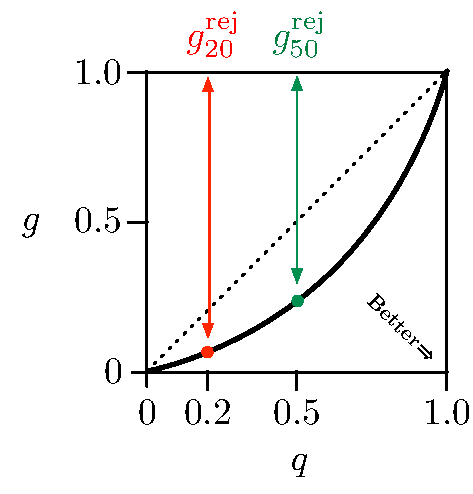
\includegraphics[width = 0.4\columnwidth]{figures/roc_curve}
}
$\quad$
\subfloat{
\label{fig:truth_overlap}
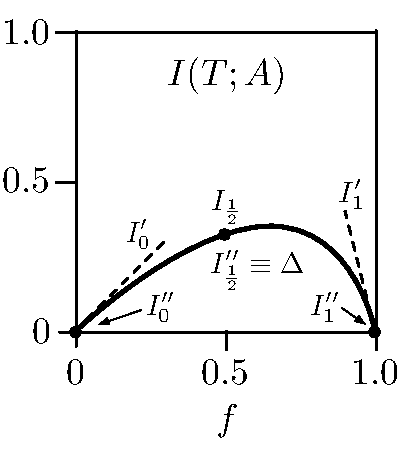
\includegraphics[width = 0.4\columnwidth]{figures/truth_overlap}
}
\caption{(a) Five ROC Curve benchmark points.  (b) Six mutual information benchmark values.}
\end{figure}

An alternative way to quantify discrimination power is through mutual information, which counts the number of ``bits'' of information gained from measuring a discriminant variable (see \cite{Larkoski:2014pca}).  Given a sample with quark fraction $f \in [0,1]$ and gluon fraction $(1-f)$, the mutual information with the truth (a.k.a. the truth overlap) is:
\be
I(T;A) = \int \df a \left(f \, p_q(a) \log_2 \frac{p_q(a)}{p_{\rm tot}(a)} + (1-f) \, p_g(a) \log_2 \frac{p_g(a)}{p_{\rm tot}(a)}   \right),
\ee
where $p_q$ ($p_g$) is the probability distribution for quarks (gluons), and
\be
p_{\rm tot}(a) = f \, p_q(a) + (1-f) \, p_g(a).
\ee
The minimum value of $I(T;A)$ is $0$ (no discrimination) and the maximum value is
\be
I(T;A)_{\rm max} = f \log_2 \frac{1}{f} + (1-f) \log_2 \frac{1}{1-f},
\ee
which equals $1$ for $f = \frac{1}{2}$.

The choice $f = 1/2$ was used in \Ref{Larkoski:2014pca}, $I(T;A)\big|_{f = \frac{1}{2}} \equiv I_{\frac{1}{2}}$, though other $f$ choices are plausible.  The first derivative at $f = 1/2$ is not particularly enlightening, but the second derivative is sometimes referred to as the classifier separation:
\be
- \frac{\log 2}{4} \frac{\partial^2 I(T;A)}{\partial f^2} \Big|_{f = \frac{1}{2}} \equiv I''_\frac{1}{2} = \frac{1}{2} \int \df a \frac{\left(p_q(a) - p_g(a)\right)^2}{p_q(a) + p_g(a)}.
\ee
At $f = 0$ and $f = 1$, the mutual information itself is zero, but the derivatives are related to other concepts in statistics:
\be
\frac{\partial I}{\partial f} \Big|_{f = 0} \equiv I'_0 = \int \df a \, p_q(a)  \log_2 \frac{p_q(a)}{p_g(a)}, \qquad - \log 2 \,  \frac{\partial^2 I}{\partial f^2} \Big|_{f = 0} \equiv I''_0 = \int \df a \,  \frac{p_q(a)^2}{p_g(a)},
\ee
\be
- \frac{\partial I}{\partial f} \Big|_{f = 1} \equiv I'_1 = \int \df a \, p_g(a) \log_2 \frac{p_g(a)}{p_q(a)}, \qquad - \log 2 \, \frac{\partial^2 I}{\partial f^2} \Big|_{f = 1} \equiv I''_1 = \int \df a \, \frac{p_g(a)^2}{p_q(a)}.
\ee
The first derivative is sometimes called relative entropy and the second derivative is sometimes called discrimination significance.  We will quote all six of the above values, visualized in \Fig{fig:truth_overlap}:
\be
\{I_\frac{1}{2}, I''_{\frac{1}{2}}, I'_0, I''_0, I'_1, I''_1 \},
\ee










\bibliographystyle{JHEP}
\bibliography{lh2015_qg}

\end{document}
